\section{Greedy Dynamic Quadruped Gait Generation}

\subsection{Terrain Representation}

\begin{outline}
  Explain how you represent the terrain for CNN input.
\end{outline}



%%%%%%%%%%%%%%%%%%%%%%%%%%%%%%%%%%%%%%%%%%%%%%%%%%%%%%%%%%%%%%%%%%%%%%%%%%%%%%%%%%%%%%%%%%%%%%%%%%%%
\subsection{Network Architecture}

\begin{outline}
  Detail the architecture of the CNNs used for contact configuration and footstep target/swing duration evaluation.
\end{outline}


The footstep evaluation neural network architecture is shown in \autoref{fig:diagram-nn-architecture} accomplishes a similar task to ContactNet \cite{bratta_contactnet_2024}. It takes in terrain and state information and ranks each of the possible footstep positions. This network uses a multi-modal middle fusion architecture. This architecture was chosen to effectively combine the spatial features from the terrain data with the contextual features from the robot state data, while still maintaining flexibility in case re-training is needed \cite{feng2021deep}. The terrain data is processed through a series of convolutional layers, while the robot state data is processed through fully connected layers. The outputs of these two branches are then concatenated and passed through additional fully connected layers to produce the final output, which consists of preference ratings for each potential footstep position.

\begin{todo}
  Discuss gait net architecture
\end{todo}

\begin{todo}
  Discuss training procedure
\end{todo}

\begin{figure}
  \centering
  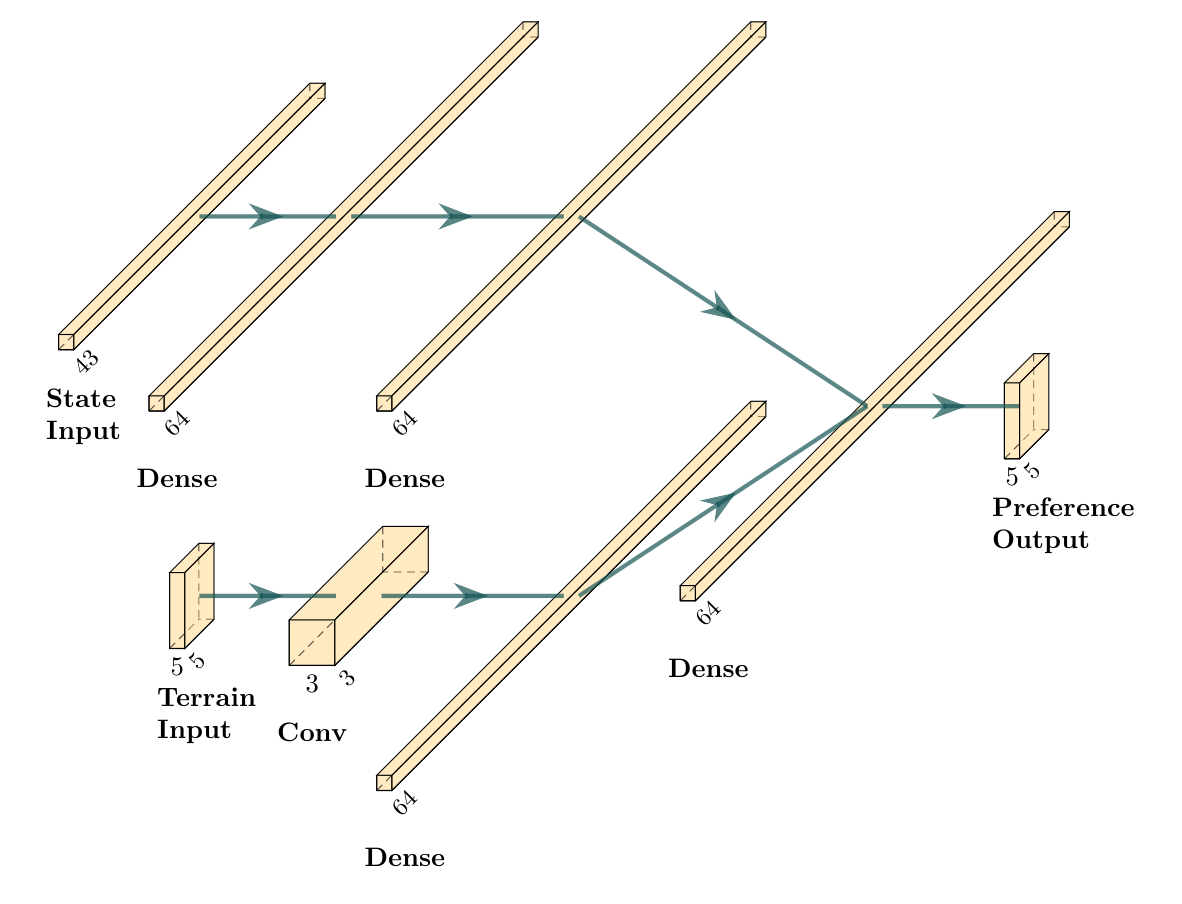
\includegraphics[width=0.5\linewidth]{images/diagrams/nn-architecture.png}
  \caption{Footstep evaluation neural network architecture.}
  \label{fig:diagram-nn-architecture}
\end{figure}

%%%%%%%%%%%%%%%%%%%%%%%%%%%%%%%%%%%%%%%%%%%%%%%%%%%%%%%%%%%%%%%%%%%%%%%%%%%%%%%%%%%%%%%%%%%%%%%%%%%%
\subsection{Greedy Decision-Making}

\begin{outline}
  Elaborate on the greedy selection process for choosing the highest-scoring, feasible action.
\end{outline}
